\chapter{Development}
\label{ch.development}

	The development of this undergraduate dissertation consists of two main contributions.
	\autoref{sec.low-level-comm} presents the most extensive part of the work. That section
	discusses how \mppa hardware was used to provide three communication abstractions for
	\nanvix \textit{\hal} and the challenges and solutions encountered during development.
	Next, \autoref{sec.user-level-comm} presents a standard view of the user services
	developed for \nanvix \microkernel that make use of the low-level interface.

	\section{Low-Level Communication}
	\label{sec.low-level-comm}

		\nanvix \textit{\hal} provides the inter-cluster communication module to allow separate
		clusters to exchange information.
		This module consists of three abstractions, named \sync, \mailbox, and \portal.
		These abstractions provide more precise, easy-to-use, scalable, and easily
		portable mechanisms for different architectures~\cite{wentzlaff_fleets:_2011}.
		Above them, it is possible to create from the most straightforward services, such
		as synchronization and data exchange, to more elaborate services
		like \shm, \posix Semaphore, and \rmem~\cite{penna:rmen}.
		Expected behavior can be simulated by both types of calls, synchronous or
		asynchronous, depending only on hardware support.
		Motivated to expose better \qos control to the upper layers, we decouple small data
		transfers from large ones, \ie \mailbox and \portal.
		Note that it would be possible to use an \noc for each abstraction if the hardware supported it.
		We did not do this in \mppa because \cnoc only provides the transfer of 64-bit values.
		
		This section is organized as follows.
		\autoref{sec.mppa-hardware-resources} clarifies the use of \mppa hardware resources.
		\autoref{sec.general-concepts} covers commonalities between all abstractions.
		\autoref{sec.sync-abs},
		\autoref{sec.mailbox-abs}, and
		\autoref{sec.portal-abs}
		conceptually present each of the abstractions, encompassed problems, and 
		implementation details.

		\subsection{\mppa Hardware Resources}
		\label{sec.mppa-hardware-resources}

			The realization of low-level communication mainly depends on two \mppa features.
			First, the interrupt system allows the configuration of handlers for messages
			received and sent through \noc. Interrupts enable asynchronous operations,
			which is a vital point in a microkernel-based operating system where the
			master cannot be blocked waiting for a single communication to complete.
			If it were not possible to perform at least asynchronously receiving
			data/signals, upper layers would face severe performance issues. Second,
			\dma is the mediator of all communications, either synchronous or asynchronous.
			At this point, a \hypervisor virtualizes the \dma, separating it into two global
			logical structures, one for \cnoc and one for \dnoc. Each structure groups
			registers for the send/receive configuration, and bit fields indicating which
			slots generated an interrupt. The \hypervisor runs on \rms and asynchronously
			controls read/write permissions of virtualized registers.

			The control made by the \hypervisor does not include allocation or manipulation
			of resources. Consequently, we manually control allocation through bit fields.
			If an operation does not comply with this control, a negative value is returned,
			indicating the error, \eg allocation of a resource that is already in use.
			Thus, we do not inflict undesired costs by shifting responsibility for handling
			the error to the upper layer, \eg waiting for the release of a resource.
			Manipulation involves procedures for configuring the \dma with proper
			permissions and ensuring cache consistency of operations. Finally, it is
			noteworthy that there is no concurrency control over the commented
			structures so as not to inflict a cost over the microkernel approach.
			If the \nanvix \hal is used to develop a monolithic \os, it should be
			concerned with ensuring atomic operations.

			The \dma coordinates three interruption lines. Two of these are used by
			\dnoc to notify the data receipt and completion of data sending by a
			$\mu$~thread. \cnoc only uses one line for receiving signals because
			sending a signal (64-bit value) is explicitly performed by the core.
			For each interrupt line, there is a specific handler, but they all
			execute a similar algorithm. \autoref{alg.noc-handler} exemplifies
			the behavior of an \noc handler. Because the line only notifies what
			type of interrupt, it is the responsibility of the handler to search
			the resources of each interface looking for who triggered the interrupt.
			The handlers are reentrant to avoid loss of interrupts. Due to the
			microkernel approach, concurrency issues are softened because only
			the master handles interrupts.

			\begin{algorithm}[!tb]
				\caption{Simplified NoC Handler Algorithm.}%
				\label{alg.noc-handler}%
				\begin{algorithmic}[1]
					\Require $status[M_{Interfaces}][N_{Resources}]$, interrupt status of a resource.
					\Require $handlers[M_{Interfaces}][N_{Resources}]$, interrupt handler of a resource.
					\Procedure{noc\_handler}{}
					\For {$i \in [1, M_{Interfaces}]$}
						\For {$j \in [1, N_{Resources}]$}
							\If {$status[i][j] == Interrupt Triggered$}
								\State {$\Call{clean\_status}{i, j}$}
								\State {$\Call{handlers[i][j]}{i, j}$}
							\EndIf
						\EndFor
					\EndFor
					\EndProcedure
				\end{algorithmic}%
				\fonte{Developed by the Author.}%
			\end{algorithm}

			\noc interfaces have two identifiers, one physical (physical ID) and the
			other logical (logical ID). The hardware uses the physical IDs in the
			process of data routing through \noc. Each physical ID is associated with
			a Logical ID to enable the identification of \noc nodes outside the \hal.
			Logical IDs primarily serve to disassociate the node identification from
			the architecture that implements the \hal. \autoref{tab.noc-node-id}
			presents the proposed mapping for \mppa clusters. Each row has one of
			three groups of existing \noc nodes (first column), grouped by type of
			the clusters. Within each group, we have a set of physical identifiers
			(second column) that are mapped 1 to 1 to logical identifiers (third column).
			For example, the \iocluster 0 constitutes 4 \noc interfaces, where they are
			mapped as follows: $128 \to 0$, $129 \to 1$, $130 \to 2$, and $131 \to 4$.
			This mapping is a more natural form to identifiers the \noc nodes through
			different architectures.

			\begin{table}[!tb]
				\centering%
				\caption{NoC Interface Identification.}%
				\label{tab.noc-node-id}%

				\begin{tabular}{l|l|l|}
					\cline{2-3}
															   & \textbf{Physical ID} & \textbf{Logical ID} \\ \hline
					\multicolumn{1}{|l|}{\textbf{\iocluster0}} & 128-131              & 0-3                 \\ \hline
					\multicolumn{1}{|l|}{\textbf{\iocluster1}} & 192-195              & 4-7                 \\ \hline
					\multicolumn{1}{|l|}{\textbf{\cclusters}}  & 0-15                 & 8-23                \\ \hline
				\end{tabular}

				\fonte{Developed by the Author.}%
			\end{table}

			The sender needs to know which logical ID the receiver will use to perform
			a communication. For instance, if the receiver sets up receiving on one
			\dnoc resource and the sender sends it to another, even if the ID is correct,
			the \dma will not notify the receiver. For this reason, the receive slots
			of the \cnoc and \dnoc have been partitioned by abstraction. Within a
			partition, each slot is statically mapped to a logical ID, \eg 0 to 23 mappings.
			In contrast, transfer channels can be dynamically allocated. However,
			an essential concept of Nanvix HAL is to provide the resources required for
			a given operation without performing additional optimizations. Thus, the
			transfer channels were also partitioned by abstraction so that they are
			reserved for an entire job. \autoref{tab.noc-resources} presents each
			abstraction, identified by the rows, and the partitioning of the resources
			of each \noc, identified by the columns. Since \sync does not exchange
			arbitrary data, no resources have been reserved in \dnoc. It is worth
			noting that even without using all existing slots, improving
			programmability by not having to specify communication features is a
			strength of abstraction design.

			% To perform the communication between two clusters, it is necessary that the
			% sender knows which resource the receiver will use.
			% For this reason, the receive slot range of \cnoc and \dnoc are partitioned
			% by abstraction, as can be seen in \autoref{tab.noc-resources}.
			% Within a partition, each slot is associated with a cluster's logical ID.
			% 	\todo{"On the another hand" does not make sense AGAIN.}
			% On the other hand, the transmitters use sending channels that need to
			% be reserved during the entire operation.
			% 	\todo{Explain the table.}
			% Thus, \autoref{tab.noc-resources} also shows the partition of the
			% sending channels for each abstraction.

			\begin{table}[!tb]
				\centering%
				\caption{Partitions of NoC resources by abstraction.}%
				\label{tab.noc-resources}%

				\begin{tabular}{l|l|l|l|l|}
					\cline{2-5}
															& \multicolumn{2}{c|}{\textbf{\cnoc}}          & \multicolumn{2}{c|}{\textbf{\dnoc}}          \\ \cline{2-5}
															& \textbf{RX Slot ID} & \textbf{TX Channel ID} & \textbf{RX Slot ID} & \textbf{TX Channel ID} \\ \hline
					\multicolumn{1}{|l|}{\textbf{\mailbox}} & 0-23                & 0                      & 0-23                & 1-3                    \\ \hline
					\multicolumn{1}{|l|}{\textbf{\portal}}  & 24-47               & 1-2                    & 24-47               & 4-7                    \\ \hline
					\multicolumn{1}{|l|}{\textbf{\sync}}    & 48-71               & 3                      & -                   & -                      \\ \hline
				\end{tabular}

				\fonte{Developed by the Author.}%
			\end{table}

			Finally, we were able to remove almost all dependency on the software
			stack provided by Kalray. However, by eliminating communication
			libraries, the lack of documentation of hardware virtualization,
			and functional examples of communication, limitations have arisen
			in the transfer of data through \dnoc. In summary, it was not possible
			to correctly configure existing $\mu$~threads in the \dma for asynchronous
			transfer, making it a future job. However, this limitation did not
			impact on the design of abstractions, requiring only that the master
			core waste time transferring data manually.

		\subsection{General Concepts of Communication Abstractions}
		\label{sec.general-concepts}

			Technically, \nanvix \hal does not know what types of applications
			or kernels have used it. Thus, we must ensure a standard behavior
			that does not affect the functionality of the upper layer. The
			microkernel specifically restricts the master core from being
			almost always available to handle slave requests. Therefore,
			interfaces export only asynchronous calls. This decision forces
			the upper layer, if desired, to create synchronous calls that
			call the wait function right after the asynchronous operation.
			Thus, at the microkernel level, we can ensure that the master
			sets or executes asynchronous functions and notifies blocked
			slaves. In \mppa, spinlocks perform synchronization between the
			master and the slaves. Upon completion of an operation, the master
			releases the lock for the slave to continue its execution.

			However, the limitation of the \dma, described in
			\autoref{sec.mppa-hardware-resources} adds an aggravation to the
			transfer operations of the mailbox and portal abstraction.
			In these abstractions, there is a flow control where the receiver
			must notify the sender, permitting him to transfer the data. This
			behavior can cause the master to lock while waiting for permission.
			The concept of lazy sending was introduced to circumvent this
			problem. \autoref{alg:lazy-transfer} illustrates the behavior of
			lazy transfer, where the master saves the parameters if not
			allowed and will handle other requests. Upon receiving permission
			from the receiver, the interrupt handler identifies the resource,
			actually sends the data and releases the slave that requested the
			send. This algorithm ensures that the master is always doing useful
			operations and never crashes the entire system.

			\begin{algorithm}[!tb]
				\caption{Simplified Lazy Transfer Algorithm.}%
				\label{alg:lazy-transfer}%
				\begin{algorithmic}[1]
				\Require $resources$, Abstraction Resource Table

				\Algphase{Configures data transfer.}

					\Procedure{async\_write}{$id, message, size$}
						\State {$resources[id].message \gets message$}
						\State {$resources[id].size \gets size$}
						\If {$resources[id].has\_permission$} 
							\State {$\Call{do\_lazy\_transfer}{id}$}
						\Else
							\State {$resources[id].is\_waiting \gets True$}
						\EndIf
					\EndProcedure%

				\Algphase{Receives permission.}

					\Procedure{abstraction\_handler}{$id$} 
						\If {$resources[id].is\_waiting$} 
							\State {$\Call{do\_lazy\_transfer}{id}$} 
						\Else
							\State {$resources[id].has\_permission \gets True$}
						\EndIf
					\EndProcedure%

				\Algphase{Transfers the data.}

					\Procedure{do\_lazy\_transfer}{$id$} 
						\State {$resources[id].is\_waiting \gets False$}
						\State {$resources[id].has\_permission \gets False$}
						\State {$\Call{transfer\_data}{resources[id].message, resources[id].size}$} 
						\State {$\Call{unlock}{resources[id].lock}$}                                \Comment{Releases slave core.}
					\EndProcedure%

				\end{algorithmic}%

				\fonte{Developed by the Author.}%
			\end{algorithm}

			Finally, abstraction interfaces follow a convention to distinguish
			between receiver and sender roles. Receivers use functions with
			\texttt{create}, \texttt{unlink}, \texttt{aread}, and \texttt{wait}
			suffixes. Senders, in turn, use functions with \texttt{open},
			\texttt{close}, \texttt{awrite/signal}, and \texttt{wait} suffixes.
			Because the \texttt{wait} function is shared, the abstraction must
			distinguish the role by the resource identifier. Discriminating the
			nature of operations helps both the user, being entirely intuitive,
			and implementing HAL by explaining what features will be needed.

			% Por fim, como já comentado anteriormente, o Nanvix HAL não realiza nenhum tipo de multiplexação dos recursos físicos do hardware.
			% A quantidade de recursos de comunicação disponíveis é diretamente relativa a quantidade de recursos físico para realizar uma dada operação.
			% A tabela 4 mostra quais recursos físicos são necessário para cada abstração e a quantidade total de abstrações simultaneas que podem existir.
			% Por exemplo, a criação de um portal precisa de um slot de recebimento da DNoC e 1 canal de transmissão da CNoC.
			% As quantidades são baixas devido aos poucos canais de transmissão, porém quem deve se preocupar com a multiplexação dos recursos deve ser da camada superior.

			% \begin{table}[!tb]
			% 	\centering%
			% 	\caption{Physical requirements by abstraction.}%
			% 	\label{tab.abstractions-amount}%

			% 	\begin{tabular}{l|l|l|l|l|l|l|}
			% 		\cline{2-7}
			% 												& \multicolumn{3}{c|}{\textbf{Create}}  & \multicolumn{3}{c|}{\textbf{Open}}                              \\ \cline{2-7}
			% 												& \multicolumn{1}{|c|}{\textbf{RX}}
			% 												            & \multicolumn{1}{|c|}{\textbf{TX}}
			% 															            & \multicolumn{1}{|c|}{\textbf{Available}}
			% 																		                & \multicolumn{1}{|c|}{\textbf{RX}}
			% 																				                    & \multicolumn{1}{|c|}{\textbf{TX}}
			% 																				        			            & \multicolumn{1}{|c|}{\textbf{Available}} \\ \hline
			% 		\multicolumn{1}{|l|}{\textbf{\mailbox}} & 1 (\dnoc) & 1 (\cnoc) & 1             & 1 (\cnoc) & 1 (\dnoc) & 4                                        \\ \hline
			% 		\multicolumn{1}{|l|}{\textbf{\portal}}  & 1 (\dnoc) & 1 (\cnoc) & 2             & 1 (\cnoc) & 1 (\dnoc) & 4                                        \\ \hline
			% 		\multicolumn{1}{|l|}{\textbf{\sync}}    & 1 (\cnoc) & 0         & 24            & 0         & 1 (\cnoc) & 1                                        \\ \hline
			% 	\end{tabular}

			% 	\fonte{Developed by the Author.}%
			% \end{table}

		\subsection{Sync Abstraction}
		\label{sec.sync-abs}

			\textit{Synchronization Abstraction}, called \sync, provides the
			basis for cluster synchronization across distributed barriers.
			Its behavior is analogous to \posix Signals abstraction, but
			notifications do not carry information, they are only for synchronization.
			\sync defines two synchronization modes, \texttt{ALL\_TO\_ONE} and
			\texttt{ONE\_TO\_ALL}. In both modes separates the clusters between
			a single master node (\texttt{ONE}) and one or more slave nodes
			(\texttt{ALL}). \autoref{fig:sync-all-to-one} illustrates the
			\texttt{ALL\_TO\_ONE} mode, where the master node waits blocked for
			the $N$ notifications coming from the slaves. In contrast,
			\autoref{fig:sync-one-to-all} pictures the \texttt{ONE\_TO\_ALL} mode,
			where the master notifies the $N$ slaves, releasing them from the lock.
			The sender nodes are responsible for sending a signal and never will
			block. Receiver nodes are responsible for waiting for all notifications
			to arrive.

			\begin{figure}[!tb]
				\centering%
				\caption{Synchronization Abstraction Example.}%
				\label{fig:sync-concepts}%

				\subcaptionminipage[fig:sync-all-to-one]%
					{.45\linewidth}%
					{N Slaves notify the Master (\texttt{ALL\_TO\_ONE}).}%
					{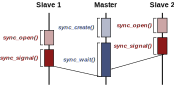
\includegraphics[width=\linewidth]{sync-all-to-one.pdf}}%
				\hspace{1cm}%
				\subcaptionminipage[fig:sync-one-to-all]%
					{.45\linewidth}%
					{The Master notifies N Slaves (\texttt{ONE\_TO\_ALL}).}%
					{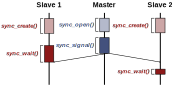
\includegraphics[width=\linewidth]{sync-one-to-all.pdf}}%

				\fonte{Developed by the Author.}%
			\end{figure}

			\subsubsection{Receiver Side Implementation}

% O que é a interface?
% Quais são os parâmetros para realizar uma operação?
				\autoref{code:hal-sync-receiver} introduces the Sync Interface for
				Receiver Nodes proposed for the \nanvix \hal. The parameters required
				for creating a sync point are a list of logical IDs, list size,
				and mode of synchronization. The list must always be initialized
				with the master node ID, regardless of mode. The remaining identifiers,
				provided they have no repetition, can be in any order. The other
				functions use the abstraction identifier returned by the create
				function. If any parameters are in disagreement or invalid, a
				negative value is returned indicating the error, \eg nodes pointer
				equal to \texttt{NULL}.

% Quais recursos são necessário para cada tipo de operação, envio e recebimento?
				Receipt of notifications requires booking one \cnoc receiving slot
				related to the Master ID. This relation eliminates the conflict of
				using a same slot across different synchronization settings.
				Consequently, a node cannot be the master in two simultaneous operations.
				Thus, the total of \sync created simultaneously is equal to the number
				of existing nodes, \ie 24 in \mppa. In \ioclusters, this total is
				multiplied by the number of available NoC interfaces, \ie 24 per \dma.
				A 64-bit mask, created from sender node IDs, configures the receiving
				slot. Bits positioned on nodes IDs are 0. When receiving a signal,
				\dma performs an \textit{OR-bitwise} with the previous value. When
				all bits become 1's, \dma clears the register and triggers an interrupt.

% Como as operações funcionam?
				A vector of internal structures controls the operations. Each structure
				is reserved for a physical slot and holds control flags, the initial mask,
				and a spinlock. \hal checks for discrepancies in IDs, control flags, or
				parameters when creating, waiting, or unlinking a \sync. Finally,
				the spinlock is used to synchronize the operation with slave cores.
				On a microkernel-based system, the master core configures \sync, and
				the slave waits for the spinlock release. The interrupt handler of the
				\sync identifies the structure and releases the lock. The lack of cache
				coherence does not affect spinlocks because instructions that guarantee
				the atomicity are used to implement the lock.

% Como foi resolvido o problema de multiplos nós nos IOs? PRECISA FALAR? DARIA PRA ARRUMAR ISSO NO CÓDIGO FORÇANDO QUE O ID[1] FOSSE O ID LOCAL (CASO NAO FOR O MESTRE).
				% A lista de nós foi projetada para utilizar os IDs das interfaces NoCs
				% ao invés dos IDs dos Cluster para não desperdiçar as DMAs extras existentes nos Cluster I/O.

\begin{listing}[!tb]
\caption{Nanvix HAL: Sync Interface for Receiver Node.}
\label{code:hal-sync-receiver}
\begin{minted}{c}
/**
 * @brief Allocates and configures the receiving side of
 * the synchronization point.
 */
int sync_create(const int *nodes, int nnodes, int mode);

/* @brief Releases and cleans receiver slot. */
int sync_unlink(int syncid);

/* @brief Waits a signal. */
int sync_wait(int syncid);
\end{minted}
\fonte{Developed by the Author.}
\end{listing}

			\subsubsection{Sender Side Implementation}

% O que é a interface?
% Quais são os parâmetros para realizar uma operação?
				The Sync Interface for Sender Nodes, presented by
				\autoref{code:hal-sync-sender}, uses the same create parameters for
				opening a \sync point. The standardization of parameters simplifies
				the role of a cluster in a synchronization. However, at both creation
				and opening, the local ID must be included in the list. For instance,
				a \sync opened with the local ID as master, but the mode defines
				\texttt{ALL\_TO\_ONE} behavior. This discrepancy will return an error
				because the master should be the notification receiver and not the
				sender. The rest of the implementation follows what was already
				explained in the previous section.

% Quais recursos são necessário para cada tipo de operação, envio e recebimento?
% Como as operações funcionam?
				Unlike the receiver, the sender needs one \cnoc transfer channel to
				open a \sync point. Due to the separation of channels described in
				the \autoref{tab.noc-resources}, a node can only open one \sync at
				a time. The node must identify the target ID and receiving slot of
				the master to emit a signal. A 64-bit value composes the mask with
				the sender node bit set to 1. The sender control structure also has
				flags to ensure the semantics of the operations. Besides, the sender
				stores, in an array of integers, all IDs of the receivers. When
				performing the notification, a signal will be sent to each target
				of this list.

\begin{listing}[!tb]
\caption{Nanvix HAL: Sync Interface for Sender Node.}
\label{code:hal-sync-sender}
\begin{minted}{c}
/**
 * @brief Allocates and configures the sending side of
 * the synchronization point.
 */
int sync_open(const int *nodes, int nnodes, int mode);

/* @brief Releases the transfer channel. */
int sync_close(int syncid);

/* @brief Sends a signal. */
int sync_signal(int syncid);
\end{minted}
\fonte{Developed by the Author.}
\end{listing}

		\subsection{Mailbox Abstraction}
		\label{sec.mailbox-abs}


			% The \textit{Mailbox Abstraction} allows clusters to exchange fixed-size
			% messages with each other.
			% The message was thought to be a relatively small size, usually a few hundred bytes.
			% Similarly, the operation of the \mailbox follows \posix message queue behavior.
			% For example, the message can be used to encode small operations and system
			% control signals.
			% As illustrated in \autoref{fig:mailbox}, the operation cardinality is N:1,
			% where N senders can transfer one message at a time to a receiver queue.
			% When the receiver consumes a message, it notifies the sender to ensure
			% control of the flow.

			\textit{Message Queue Abstraction}, called \mailbox, allows clusters to exchange
			fixed-length messages with each other. The message size is designed to be
			relatively small, usually a few hundred bytes. The recipient consumes these
			messages without needing to know who sent them. Similarly, mailbox operations
			follows the behavior of the \posix message queue. \autoref{fig:mailbox-concept}
			conceptually illustrates one of the ways to implement a \mailbox. The receiver
			allocates enough space to receive one message from each possible sender.
			The sender transfers the message to a predefined location.

			\begin{figure}[!tb]
				\centering%
				\caption{Mailbox Abstraction Concept.}%
				\label{fig:mailbox}%

				\subcaptionminipage[fig:mailbox-concept]%
					{.32\linewidth}%
					{Conceptual Overview.}%
					{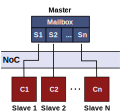
\includegraphics[width=\linewidth]{mailbox-concept.pdf}}%
				\hspace{1cm}%
				\subcaptionminipage[fig:mailbox-flow]%
					{.55\linewidth}%
					{Flow of execution: Slave sends a message, Master reads and notifies the sender.}%
					{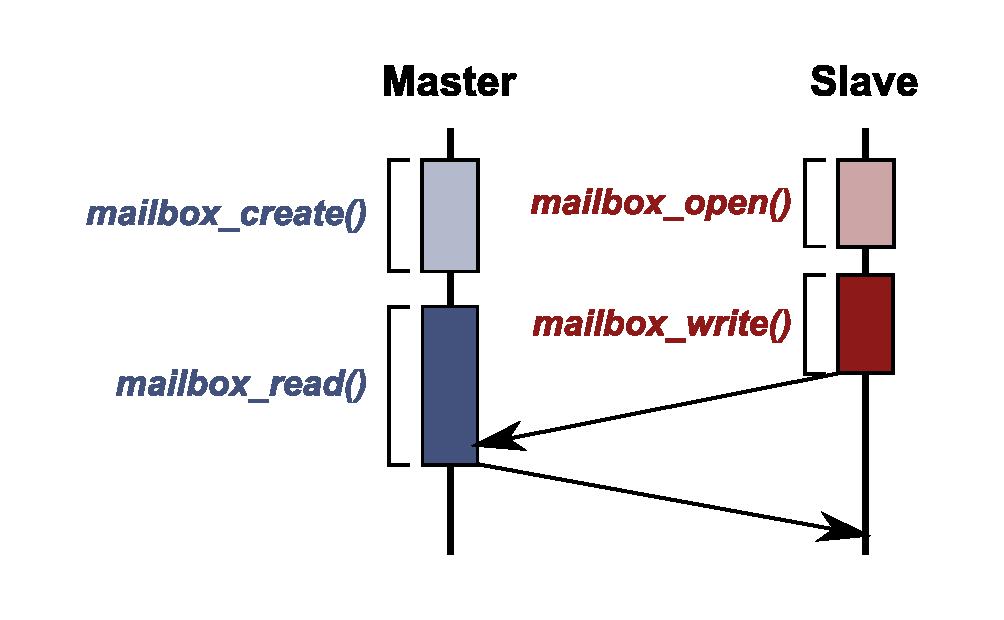
\includegraphics[width=\linewidth]{mailbox-flow.pdf}}%

				\fonte{Developed by the Author.}%
			\end{figure}

			\autoref{fig:mailbox-flow} exemplifies the communication flow between a
			receiver and a sender node. The receiver creates an empty message queue
			where senders are free to send the first message. Subsequently, in order
			not to overwrite old messages, all transmissions require the permission
			of the receiver. For this reason,  when the receiver consumes a message,
			it copies the message to the user buffer, releases the queue space, and
			notifies the sender.
			
			Theoretically, the number of messages allowed per sender can be from
			$1$ to $N$. However, \nanvix \hal statically allocates sufficient
			memory for the message queue inside the kernel. Therefore, we chose
			to allow only one message due to memory constraints presented by
			lightweight manycores. Furthermore, using one message is sufficient	for
			servers to handle requests at the \multikernel level. For instance, the
			message can be used to encode small operations and system control signals.
			
			\subsubsection{Receiver Side Implementation}

% % Interface e seus parâmetros
					\autoref{code:hal-mailbox-receiver} presents the Mailbox interface for
					Receiver Nodes. The multiples nodes in \ioclusters forces the application
					to inform the local node ID on the creation of the \mailbox. The other
					operations use the file descriptor returned by creation function.
					Consumption of a message requires the application to enter a buffer and
					message size. Although the size is constant, it is used to verify the
					integrity of the operation. Successful copying of a message will release
					the slave that performs the wait function. In the release protocol, the
					master core flushes the message to the SRAM so that the slave, when
					invalidating its cache, can read the message.
					
% % Recursos de hardware
					\mailbox is more complicated than Sync in terms of hardware resources.
					Specifically, the receiver requires one \dnoc receiving slot and one \cnoc
					transfer channel. The need for one transfer channel for the lifetime
					of the receiver limits the creation of only one mailbox per \noc node.
					The receiving slot is configured using two sizes. One for the size of
					a message, which will generate interrupts, and one for the total buffer
					size allocated for protection. The buffer is allocated within kernel
					memory with sufficient space to receive 24 messages. The message
					itself is composed of a header identifying the sender, a body containing
					the useful message, and a footer for handler control. The transfer channel,
					in turn, is used after copying the useful message to the user buffer,
					notifying the header ID.
					
% % Desafios da implementação
					Parallelism in receiving messages introduced some challenges in the
					asynchronous reading of Mailbox. Where (i) each message generates an
					interrupt, (ii) interrupts preempted by others did not find the \dnoc
					resources that issued the interrupt, and (iii) cannot verify the
					number of interrupts generated by a resource. A behavior similar to
					lazy transfer has been implemented to circumvent these difficulties.
					First, a global counter containing the total amount of messages
					received allows the receiver to copy received messages on the
					asynchronous read call. Second, if no messages are available, copying
					will be performed by the next triggered handler. Third, to solve the
					problem of preemptive interrupts, whenever a handler is triggered,
					it will traverse the message queue checking headers and footers.
					When identifying a valid message, the handler increments the counter
					and changes the footer to a specific code. This way, no message is
					lost because a single handler identifies messages not yet counted.

\begin{listing}[!tb]
\caption{Nanvix HAL: Mailbox Interface for Receiver Node.}
\label{code:hal-mailbox-receiver}
\begin{minted}{c}
/* @brief Creates a mailbox. */
int mailbox_create(int nodenum);

/* @brief Destroys a mailbox. */
int mailbox_unlink(int mbxid);

/* @brief Reads data asynchronously from a mailbox. */
ssize_t mailbox_aread(int mbxid, void * buffer, size_t size);

/* @brief Waits for an asynchronous operation to complete. */
int mailbox_wait(int mbxid);
\end{minted}
\fonte{Developed by the Author.}
\end{listing}

			\subsubsection{Sender Side Implementation}

% Interface e seus parâmetros
				\autoref{code:hal-mailbox-sender} displays the Mailbox Interface for
				Sender Nodes. Opening a mailbox requires the application to inform
				the receiver ID to allocate related resources. The send function,
				in particular, implements the concept of lazy transfer. So, the master
				core never blocks if the mailbox is not allowed to transfer the message.
				The wait function is the same function used by the receiver node where
				the slave core waits blocked until receiving the transfer permission.

				% If the sender attempts to send a message before the receiver has consumed
				% the previous message, the sender will be blocked waiting for the sender's notification.
				% In this way, flow control is guaranteed, and the sender will not overwrite
				% messages unread by the receiver.

% Recursos de hardware
				The sender implementation also requires the allocation of resources
				from both \nocs. However, the resources are opposite to the receiver,
				where it allocates one \cnoc receiving slot and one \dnoc transfer channel.
				The allocated \cnoc receiving slot is relative to the receiver ID to
				prevent conflicts among openings for distinct receivers. The transfer
				channel is dynamically allocated. Because it has fewer transfer channels
				than receiving slots, transfer channels limit mailbox openings to 4 per node.

\begin{listing}[!tb]
\caption{Nanvix HAL: Mailbox Interface for Sender Node.}
\label{code:hal-mailbox-sender}
\begin{minted}{c}
/* @brief Opens a mailbox. */
int mailbox_open(int nodenum);

/* @brief Closes a mailbox. */
int mailbox_close(int mbxid);

/* @brief Writes data asynchronously to a mailbox. */
ssize_t mailbox_awrite(int mbxid, const void * buffer, size_t size);

/* @brief Waits for an asynchronous operation to complete. */
int mailbox_wait(int mbxid);
\end{minted}
\fonte{Developed by the Author.}
\end{listing}

		\subsection{Portal Abstraction}
		\label{sec.portal-abs}

% Apresentação do portal e o conceito.
			Finally, \textit{Portal Abstraction} allows two nodes to exchange arbitrary
			amounts of data. \autoref{fig:portal-concept} presents the conceptual idea
			of the \portal, which resembles that of \posix Pipes with flow control.
			The cardinality of operations is always $1:1$, where a pair of nodes opens
			a one-way channel for data transfer. However, unlike \posix Pipes, which
			defines that the pipe exists only between two processes, the \portal allows
			the receiver to communicate with other nodes through the same channel.
			The sender, in turn, can only communicate with one node.

% Fluxo da operação
			\autoref{fig:portal-flow} exemplifies the flow control of the \portal.
			When attempting to transmit data to the receiver, the sender will block
			until the receiver can accept it. By enabling one data exchange at a time,
			the receiver sets the readout and notifies the sender. In this way,
			the flow control ensures that the receiver will not be overloaded, will
			not receive data without properly configured \dma, and will not overwrite
			previous data. Allowing communication empowers the receiver to choose which
			communications to prioritize.

			\begin{figure}[!tb]
				\centering%
				\caption{Portal Abstraction Concept.}%
				\label{fig:portal}%

				\subcaptionminipage[fig:portal-concept]%
					{.32\linewidth}%
					{Conceptual Overview.}%
					{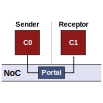
\includegraphics[width=\linewidth]{portal-concept.pdf}}%
				\hspace{1cm}%
				\subcaptionminipage[fig:portal-flow]%
					{.55\linewidth}%
					{Node 1 create a portal and notify Node 2 to transfer the data.}%
					{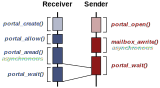
\includegraphics[width=\linewidth]{portal-flow.pdf}}%

				\fonte{Developed by the Author.}%
			\end{figure}

			\subsubsection{Receiver Side Implementation}

% Interface e seus parâmetros
				\autoref{code:hal-portal-receiver} presents the Portal Interface for
				Receiver Nodes. Like the \mailbox, the application must identify the
				local node to create a \portal. The receiver must always perform
				three operations to perform communication, i.e., \textit{allow},
				\textit{read}, and \textit{wait}. The allow function allocates one
				receiving slot relative to the given remote node, limiting one
				channel per pair of nodes. However, the permission will only be
				sent after \dma configuration by the read function. Finally, the
				node will block in the wait function until receiving the informed
				data size.

% Recursos de hardware
				A Receiver allocates one \dnoc receiving slot and one \cnoc transfer
				channel. Unlike \mailbox, the \portal has two transfer channels
				available, which allows the creation of two simultaneous portals.
				Such portals cannot communicate with the same node at the same time
				because of the choice of the same physical slot. Read sets the
				receiving slot to the buffer and size informed by the application.
				The \dma eliminates intermediate copies like Mailbox because it
				writes data directly to the application buffer. Consequently,
				control structures have also been simplified, containing only
				control flags and the spinlock for asynchronous operations.

\begin{listing}[!tb]
\caption{Nanvix HAL: Portal Interface for Receiver Node.}
\label{code:hal-portal-receiver}
\begin{minted}{c}
/* @brief Creates a portal. */
int portal_create(int local);

/* @brief Destroys a portal. */
int portal_unlink(int portalid);

/* @brief Allow sender to transfer data. */
int portal_allow(int portalid, int remote);

/* @brief Reads data asynchronously from a portal. */
ssize_t portal_aread(int portalid, void * buffer, size_t size);

/* @brief Waits for an asynchronous operation to complete. */
int portal_wait(int portalid);
\end{minted}
\fonte{Developed by the Author.}
\end{listing}

			\subsubsection{Sender Side Implementation}

% Interface e seus parâmetros
				\autoref{code:hal-portal-sender} presents the Portal Interface for
				Sender Nodes. When opening a \portal, the application is required to
				inform the local node ID and the receiver node ID. The local ID serves
				to distinguish the NoC interface on \ioclusters. The receiver node ID
				identifies the \cnoc receiving slot that will catch the transfer
				permission. The early allocation ensures that the permission will not
				be lost even if the permission arrives before the sender sets up the
				transfer. The transfer configuration follows the lazy transfer algorithm.

% Recursos de hardware
				The hardware resources required to open a portal are the opposite of
				resources to create. Specifically, one \cnoc receiving slot and one
				\dnoc transfer channel are required. The transfer channel is reserved
				but only used when the transfer is allowed. Due to the limitation of
				four transfer channels to the portal, a node can open only four portals
				at a time. The control structures for the sender portals contain the
				parameters needed to perform the lazy transfer and a spinlock to
				asynchronous operations.

\begin{listing}[!tb]
\caption{Nanvix HAL: Portal Interface for Sender Node.}
\label{code:hal-portal-sender}
\begin{minted}{c}
/* @brief Opens a portal. */
int portal_open(int local, int remote);

/* @brief Closes a portal. */
int portal_close(int portalid);

/* @brief Writes data asynchronously to a portal. */
int portal_awrite(int portalid, const void * buffer, size_t size);

/* @brief Waits for an asynchronous operation to complete. */
int portal_wait(int portalid);
\end{minted}
\fonte{Developed by the Author.}
\end{listing}

	\section{User-Level Communication}
	\label{sec.user-level-comm}

		The inter-cluster communication module, described in \autoref{sec.low-level-comm},
		is designed to export a standard and straightforward communication
		primitives to different lightweight manycores.
		These primitives can be used by various types of \oss and applications.
		Thus, the module is flexible enough not to impact the performance
		of the upper layers negatively.
		For this, it does not provide rich management of the exposed abstractions.

		In this scenario, the communication services of \nanvix \microkernel seek
		to provide \ipc between distinct clusters.
		Specifically, these services perform the multiplexing of the hardware
		resources and the verification of the parameters that will be passed
		on the communication primitives.
		Due to the Master-Slave model, the responsibility of protecting,
		manipulating, and configuring \hal resources is of the master core.
		The slave core will request operations through the system call interface,
		passing the necessary information to the master.

		Considering that the abstractions make up the fundamental elements of
		the construction of more complex services, the \microkernel services
		were responsible for the management and multiplexing of the finite
		resources for the many cores of a cluster.
		In total, there are three communication services in the \nanvix \microkernel,
		each associated with an abstraction of the communication module,
		analogously named \sync, \mailbox, and \portal services.
		These services must take into account the memory constraints and the
		Master-Slave model chosen for the \microkernel.

		The impacts of the Master-Slave model, protection, management and manipulation 
		operations are similar to all services.
		Thereat, the following sections provide an overview of these topics punctuating 
		the differences of each service.

		They will be provided through interfaces that function as wrappers
		for the \hal abstraction functions.
		In the implementation of these interfaces, there will be a mapping
		between low-level identifiers, associated with \hal resources,
		and high-level identifiers, associated with resource protection structures.

		\subsection{Impacts of the Master-Slave Model}

			Master-Slave model defines that the master core must exclusively manipulate
			the internal structures of the \os. For this, each service has generic and
			straightforward structures that hold control flags, parameters for resource
			identification, and storage of physical descriptors returned by \hal. Thus,
			the system call interface separates the functions of the services into two
			sets of functions. The first set is the system calls that request a particular
			operation. The second set is functions that operate on the internal structures
			and communicate with the \hal level. The master executes almost exclusive
			the second set, except for the wait functions, which the slave performs entirely.

			The system call set of functions follows the \texttt{kernel\_\textit{abstraction}\_\textit{operation}}
			notation. Its responsibilities are to find out which logical ID is attached to
			the local node, if there is more than one, and perform the possible sanity
			checks on the slave side. The internal set of functions follows the
			\texttt{k\textit{abstraction}\_\textit{operation}} notation. Internally, it
			is used by the system call engine to perform protection, handling, and
			multiplexing services. 

			The requirement of the slave to perform wait functions is because the master
			cannot block indefinitely waiting for an operation. At this point, the slave
			must access the internal structure of the \os to query the physical descriptor
			for access to the \hal spinlock. So, the master updates local memory whenever
			a modification is made, and the slave invalidates its cache to ensure structure
			coherence.

		\subsection{Protection and Management}

			Protection and management operations involve two phases, the slave and the master phase.
			In the slave phase, all problems that could be detected before requesting the operation
			to the master are checked.
			For instance,
			(i) valid file descriptors,
			(ii) non-null buffer pointers,
			(iii) buffer sizes within the stipulated limit, and
			(iv) the semantics of services, e.g., synchronization with itself.

			The master phase performs the same checks as the slave and has the
			responsibility to check the semantics of operations on a given resource.
			Specifically, the master
			(i) identifies multiple creations/openings
			(ii) checks for conflicting operations, e.g., writing to read-only resources,
			(iii) measures communication time and total number of bytes transmitted/received, and
			(iv) interacts with Nanvix HAL detecting errors.

		\subsection{Multiplexing}

			The Identification of creations/openings with the same arguments
			allows multiple slaves to use the same resource at different times.
			For this, the internal structures of the \os keep, as simply as possible,
			the arguments used to create/open a service. When the same arguments are
			identified, a reference counter increments. The master sets the resource
			to busy when prompted for a read/write. A second slave who wants to read/write
			 will be prevented until the previous operation is completed. The resources
			 of the \hal will only be released when all references are removed.

		\subsection{Input/Output Control}

			The \mailbox and \portal services have a particular system call denominated
			\ioctl. The \ioctl grants the implementation of operations that cannot be
			expressed by regular system calls. In the case of communication services,
			we implement two types of operations to query some informações about the
			transmissions performed. The first operation, named \texttt{IOCTL\_GET\_VOLUME},
			queries the current number of bytes transmitted/received from a service.
			The second operation, named \texttt{IOCTL\_GET\_LATENCY}, queries the sum
			of measured communication latencies by the difference of two clock readings.
			This system call may be extended in the future to introduce new features
			without causing changes to current interfaces.

		\subsection{Validation and Correctness Tests}

			Validation and correctness testing of the implementation of services was
			performed through two sets of unit tests, \textit{API} and \textit{FAULT}
			tests, respectively. On the one hand, \textit{API} tests create, open, and
			stimulate services with arguments within valid value ranges. On the other
			hand, \textit{FAULT} tests use arguments outside the domain range of the
			operations. The failure should generate a previously known error value.
			The tests validate any changes made by verifying all expected behaviors
			of each service.
